% !TEX encoding = UTF-8 Unicode
%%%%%%%%%%%%%%%%%%%%%%%%%%%%%%%%%%%%%%%%%
% Beamer Presentation
% LaTeX Template
% Version 1.0 (10/11/12)
%
% This template has been downloaded from:
% http://www.LaTeXTemplates.com
%
% License:
% CC BY-NC-SA 3.0 (http://creativecommons.org/licenses/by-nc-sa/3.0/)
%
%%%%%%%%%%%%%%%%%%%%%%%%%%%%%%%%%%%%%%%%%

%----------------------------------------------------------------------------------------
%	PACKAGES AND THEMES
%----------------------------------------------------------------------------------------

\documentclass{beamer}

\mode<presentation> {

% The Beamer class comes with a number of default slide themes
% which change the colors and layouts of slides. Below this is a list
% of all the themes, uncomment each in turn to see what they look like.

%\usetheme{default}
%\usetheme{AnnArbor}
%\usetheme{Antibes}
%\usetheme{Bergen}
%\usetheme{Berkeley}
%\usetheme{Berlin}
%\usetheme{Boadilla}
%\usetheme{CambridgeUS}
%\usetheme{Copenhagen}
%\usetheme{Darmstadt}
%\usetheme{Dresden}
%\usetheme{Frankfurt}
%\usetheme{Goettingen}
%\usetheme{Hannover}
%\usetheme{Ilmenau}
%\usetheme{JuanLesPins}
%\usetheme{Luebeck}
\usetheme{Madrid}
%\usetheme{Malmoe}
%\usetheme{Marburg}
%\usetheme{Montpellier}
%\usetheme{PaloAlto}
%\usetheme{Pittsburgh}
%\usetheme{Rochester}
%\usetheme{Singapore}
%\usetheme{Szeged}
%\usetheme{Warsaw}

% As well as themes, the Beamer class has a number of color themes
% for any slide theme. Uncomment each of these in turn to see how it
% changes the colors of your current slide theme.

%\usecolortheme{albatross}
%\usecolortheme{beaver}
%\usecolortheme{beetle}
%\usecolortheme{crane}
%\usecolortheme{dolphin}
%\usecolortheme{dove}
%\usecolortheme{fly}
%\usecolortheme{lily}
%\usecolortheme{orchid}
%\usecolortheme{rose}
%\usecolortheme{seagull}
%\usecolortheme{seahorse}
%\usecolortheme{whale}
%\usecolortheme{wolverine}

%\setbeamertemplate{footline} % To remove the footer line in all slides uncomment this line
%\setbeamertemplate{footline}[page number] % To replace the footer line in all slides with a simple slide count uncomment this line

%\setbeamertemplate{navigation symbols}{} % To remove the navigation symbols from the bottom of all slides uncomment this line
}

\usepackage{graphicx} % Allows including images
\usepackage{booktabs} % Allows the use of \toprule, \midrule and \bottomrule in tables
\usepackage{xeCJK}
\setCJKmainfont{SourceHanSerif-Regular}
\usepackage{color}
\usepackage{listings}
\lstset{numbers=left}
\usepackage{tikz}


%----------------------------------------------------------------------------------------
%	TITLE PAGE
%----------------------------------------------------------------------------------------

\title[nmap]{nmap} % The short title appears at the bottom of every slide, the full title is only on the title page

\author{} % Your name
\institute[计算机科学与技术学院] % Your institution as it will appear on the bottom of every slide, may be shorthand to save space
{
贵州大学 \\ % Your institution for the title page
\medskip
\textit{hnzhang1@gzu.edu.cn} % Your email address
}
\date{\today} % Date, can be changed to a custom date

\begin{document}

\begin{frame}
\titlepage % Print the title page as the first slide
\end{frame}
\begin{frame}{Overview}
\tableofcontents
\end{frame}
\section{Introduction}
\begin{frame}{Introduction}
\textcolor{red}{Nmap ("Network Mapper")} is a free and open source (license) utility for \textcolor{red}{network discovery} and \textcolor{red}{security auditing}. 
 %Nmap can perform  tasks such as:
 %\begin{itemize}
 %\item network inventory
 %\item managing service upgrade schedules
 %\item monitoring host or service uptime. 
 %\end{itemize}
 
 
 Nmap uses IP packets to determine 
 \begin{itemize}
 \item what hosts are available on the network, 
 \item what services (application name and version) those hosts are offering, 
 \item what operating systems (and OS versions) they are running, 
 \item what type of packet filters/firewalls are in use, 
 \item and dozens of other characteristics. 
 \end{itemize}
\end{frame}
\section{Host Discovery}
\begin{frame}
\center{\Huge{Host Discovery}}
\end{frame}
\subsection{基于不同协议的活跃主机发现技术}
\begin{frame}
\center{\large{基于不同协议的活跃主机发现技术}}
\end{frame}
\begin{frame}[fragile]{ARP}
ARP协议的作用是完成逻辑地址和物理地址的转换。几乎所有的网络设备都实现了ARP协议。这使得nmap在扫描同一网段的设备时,若使用基于ARP协议的方法,一般是无法防御的。
\begin{example}[命令语法]
\begin{verbatim}
nmap -PR target
\end{verbatim}
\end{example}
执行扫描时,nmap会构造一个arp询问包“who has target tell localhost”,若能收到回应,则说明目标主机target是开机状态,否则就是不活跃主机。
\end{frame}

\begin{frame}[fragile]{ICMP}
ICMP是互联网控制报文协议,用来在ip主机和路由器之间传递控制消息,比如差错报告报文和查询报文。基于ICMP的活跃主机发现技术使用的是查询报文,可使用的有3类:
\begin{enumerate}
\item 响应请求和应答(很多主机会禁ping,即阻止此类型的ICMP报文)

用来测试链路及目标主机的TCP/IP协议是否正常。
\item 时间戳请求和应答

ICMP时间戳请求允许系统向另一个系统查询当前的时间。
\item 地址掩码请求和应答(较少用)

ICMP地址掩码请求由源主机发送,用于无盘系统引导时获取自己的子网掩码。虽然RFC规定除非是地址掩码的代理,否则不能发送应答,但是有些主机在收到请求时会发送一个应答。
\end{enumerate}
\begin{example}[命令语法]
\begin{verbatim}
nmap -PE target
nmap -PP target
nmap -PM target
\end{verbatim}
\end{example}
\end{frame}
\begin{frame}[fragile]{TCP}
TCP(Transmission Control Protocol)是位于传输层的协议。
TCP是一个面向连接的协议,其特点就是在建立连接的时候会有一个三次握手的过程:
\begin{enumerate}
\item 客户端发送SYN(SEQ=x)报文给服务器端,进入SYN\_SEND状态
\item 服务器端收到SYN报文后回应一个SYN(SEQ=y)和ACK(SEQ=x+1)报文,进入SYN\_RECV状态
\item 客户端收到服务器端的SYN报文,回应一个ACK(SEQ=y+1)报文,进入Established状态。三次握手完成,连接建立。
\end{enumerate}

\end{frame}
\begin{frame}[fragile]{TCP-SYN/ACK}
基于三次握手的过程,nmap有两种扫描方式:
\begin{enumerate}
\item TCP SYN扫描

执行SYN扫描时,目标主机会认为nmap所在主是想与自己建立连接,若此端口是开放的,则会按三次握手规则进行回应,否则会回应一个RST数据包拒绝连接。
\item TCP ACK扫描

执行ACK扫描时,nmap主机直接发送ACK数据包到目标主机,这违反了三次握手机制,目标主机无法接受此数据包,只能回应RST数据包来拒绝连接。\textcolor{red}{通常情况下,目标主机上的安全机制会直接过滤掉这个无中生有的ACK数据包,这会导致nmap误以为目标主机是非活跃的。}
\end{enumerate}
\begin{example}[命令语法]
\begin{verbatim}
nmap -PS [port默认80] target
nmap -PA [port默认80] target
\end{verbatim}
\end{example}
\end{frame}

\begin{frame}[fragile]{UDP}
UDP(User Datagram Protocol)是位于传输层的协议。
UDP是一个非面向连接的协议,不能使用连接建立的过程构建扫描。当目标主机上的UDP端口收到UDP数据包时,若此端口是关闭的,则会给源端发回一个ICMP端口不可达的ICMP报文,否则就丢弃这个数据包而不做回应。基于UDP的主机发现技术缺点如下:
\begin{enumerate}
\item 不可靠

如果目标端口是开放的,nmap主机不会收到任何回应,会误以为目标主机是非活跃的。(当然,也有可能收不到回应是因为数据包在传输过程中丢失了)
\item 速度慢

RFC1812对ICMP错误报文的生成速度做出了限制。
\end{enumerate}
\begin{example}[命令语法]
\begin{verbatim}
nmap -PU  target
\end{verbatim}
\end{example}

\end{frame}

\begin{frame}[fragile]{SCTP\footnote{目前支持此协议的主机并不多}}
SCTP是位于传输层的协议,其与TCP功能类似,其通过4次握手建立连接。
\begin{enumerate}
\item 客户端发起INIT报文
\item 服务器端回应INIT-ACK(包含cookie)
\item 客户端回应COOKIE-ECHO报文
\item 服务器端回应COOKIE-ACK报文
\end{enumerate}
\begin{example}[命令语法]
\begin{verbatim}
nmap -PY  target(发送SCTP INIT数据包)
\end{verbatim}
\end{example}

\end{frame}

\begin{frame}[fragile]{IP}
IP协议是TCP/IP协议族中的核心协议,也是TCP/IP协议的载体。所有的TCP、UDP、ICMP、IGMP数据都是以IP数据包的格式进行传输的。nmap可以向目标主机发送IP数据包来检测目标主机是否活跃,可以指定所要使用的协议,若不指定则默认使用ICMP(1)、IGMP(2)、IP-in-IP(4)。需要注意的是nmap发送的这种IP数据包是空包,很容易被过滤,可以使用--data-length参数来发送添加了随机数据的数据包。
\begin{example}[命令语法]
\begin{verbatim}
nmap -PO  target
nmap -PO 1,2,4 target (TCP6 UDP17)
\end{verbatim}
\end{example}

\end{frame}
\subsection{主机发现技术的分析}
\begin{frame}
\center{\large{主机发现技术的分析}}
\end{frame}
\begin{frame}[fragile]{NMAP到底发送了什么样的数据包}
上面的命令执行之后nmap到底向目标主机发送了什么样的内容?可以使用-|,-packet-trace参数来查看。
\begin{example}[命令语法]
\begin{verbatim}
nmap -PS -|,-packet-trace www.gzu.edu.cn
\end{verbatim}
\end{example}

\end{frame}
\section{Port Scanning}
\begin{frame}
\center{\Huge{Port Scanning}}
\end{frame}
\subsection{几种不同的扫描方式}
\begin{frame}
\center{\huge{Port Scanning}}
\end{frame}
\begin{frame}{Port}
计算机通过端口来对外提供服务。每个网络设备的端口有$2^{16}$个。端口的分类:
\begin{enumerate}
\item
公认端口(well known port)

0〜1024就是公认端口,或者是说“常用端口”。这些端口上运行的服务一般都是约定俗成的。比如:web服务运行在80端口,ftp服务运行在21端口,ssh服务运行在22端口。一个正常的应用程序不应该使用公认端口。
\item
注册端口(registered port)

这部分端口号的范围是1025〜49151,实际运行的程序中,大部分在这些端口上注册监听对外提供服务。
\item
动态/私有端口(dynamic/private port)

范围是49152〜65535 。一般地,常用服务不会运行在这些端口上,但是由于这些端口不太容易引起人们的注意,一些病毒或木马程序喜欢使用这些端口。
\end{enumerate}
\end{frame}
\begin{frame}{nmap对端口状态的定义}
\begin{table}
\begin{tabular}{ll}
\toprule
\textbf{状态}&\textbf{说明}\\
\midrule
open&开放的,有服务在此端口上监听\\
closed&是可访问的,但没有服务在此端口上监听\\
filtered&无法确定是否开放,数据包可能被安全设备过滤掉了\\
unfiltered&目标端口是可以访问的,但是无法确定是open还是closed。通常只有在ACK扫描时才会出现这种状态。\\
open|filtered&无法确定端口是可以访问的还是被过滤了\\
closed|filtered&无法确定端口是关闭的还是被过滤了,通常只有在使用idle扫描时才会出现这种状态。\\

\bottomrule
\end{tabular}
\end{table}
\end{frame}
\begin{frame}[fragile]{基于TCP的SYN扫描}
SYN扫描是最为流行的一种扫描方式,同时也是nmap的默认扫描方式,\textcolor{red}{需要root权限}。这种扫描方式\textcolor{red}{速度快},通常可以在1s内扫描上千个端口,同时也\textcolor{red}{不容易被安全设备发现}。

nmap使用这种方式进行扫描时,在发送了SYN包,并收到SYN/ACK回应后,直接发送RST数据包中断连接。这样的话,一般不会在目标主机上留下痕迹。这次扫描也不会被记录到系统日志中。
\begin{table}
\begin{tabular}{ll}
\toprule
\textbf{目标主机应答}&\textbf{端口状态}\\
\midrule
ACK/SYN&open\\
RST&closed\\
没有应答&filtered\\
ICMP无法抵达&filtered\\
\bottomrule
\end{tabular}
\end{table}
\begin{example}[命令语法]
\begin{verbatim}
nmap -sS target
\end{verbatim}
\end{example}
\end{frame}
\begin{frame}[fragile]{基于TCP的Connect扫描}
这种方式和基于SYN的扫描很像,只是本方式\textcolor{red}{完成了三次握手},并且\textcolor{red}{不需要root权限}。
\begin{block}{命令语法}
\begin{verbatim}
nmap -sT target
\end{verbatim}
\end{block}
\end{frame}

\begin{frame}[fragile]{基于UDP扫描}
UDP扫描的速度很慢。UDP程序通常不会对nmap发送的空数据包产生回应,这就需要nmap在使用不同协议时,构造不同的数据包,比如使用SNMP和DHCP请求,所使用的数据包就完全不同。nmap将这些数据包格式存储在Nmap-service-probes中。
\begin{table}
\begin{tabular}{ll}
\toprule
\textbf{目标主机应答}&\textbf{端口状态}\\
\midrule
任意UDP应答&open\\
ICMP端口无法抵达(类型3,代码3)&closed\\
目标主机没有应答&open|filtered\\
ICMP无法抵达(类型3,代码1,2,9,10,13)&filtered\\
\bottomrule
\end{tabular}
\end{table}
\begin{example}[命令语法]
\begin{verbatim}
nmap -sU target
\end{verbatim}
\end{example}
\end{frame}

\begin{frame}[fragile]{基于TCP的FIN扫描}
nmap向目标主机发送一个TCP FIN数据包。根据RFC793的规定,对于关闭的端口,目标系统应该返回RST标志。
\begin{block}{命令语法}
\begin{verbatim}
nmap -sF target
\end{verbatim}
\end{block}
\end{frame}

\begin{frame}[fragile]{基于TCP的NULL扫描}
nmap向目标主机发送一个不包含任何标志的TCP数据包。根据RFC793的规定,对于关闭的端口,目标系统应该返回RST标志。
\begin{block}{命令语法}
\begin{verbatim}
nmap -sN target
\end{verbatim}
\end{block}
\end{frame}

\begin{frame}[fragile]{基于TCP的Xmas Tree扫描}
nmap向目标主机发送一个含有FIN、URG、PUSH标志的数据包。根据RFC793的规定,对于关闭的端口,目标系统应该返回RST标志。
\begin{block}{命令语法}
\begin{verbatim}
nmap -sX target
\end{verbatim}
\end{block}
\end{frame}

\begin{frame}[fragile]{idle扫描}
这种方式下,相当于存在一个代理,其流程如下所示。
\begin{enumerate}
\item
检测第三方(代理)的IP ID值,并记录
\item
构造一个源地址为第三方的数据包,并发送给目标主机
\item
目标主机与第三方通信
\item
检测第三方的IP ID值
\end{enumerate}


\center{
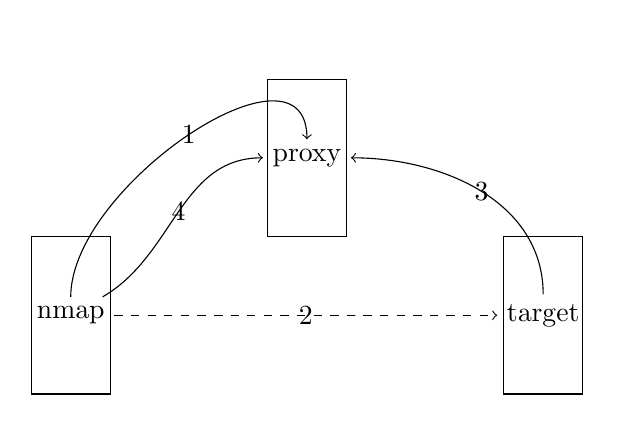
\begin{tikzpicture}
\draw (0,0) rectangle (1,2) node(n) at(0.5,1){nmap};
\draw (3,2) rectangle (4,4) node(p) at(3.5,3){proxy};
\draw (6,0) rectangle (7,2) node(t) at(6.5,1){target};

\draw [->] (n) to[out=90,in=90] node{1} (p);
\draw [->,dashed] (n) to[out=0,in=180] node{2} (t);
%\draw [->] (p) to[out=0,in=180] (t);
\draw [->] (t) to[out=90,in=360] node{3} (p);
\draw [->] (n) to[out=30,in=180] node{4} (p);
\end{tikzpicture}
}

\end{frame}
\begin{frame}{idle扫描II}
将第4步与第一步记录的IP ID值进行比较,应该增加了1或2. 如果是增加了1, 说明第三方主机在此期间并未向外发送数据包,此时认为目标主机的端口是关闭的;若增加了2, 说明对外发送过数据包,说明目标主机的端口是开放的。
\begin{block}{idle扫描的不足}
\begin{itemize}
\item
耗时长

远长于SYN扫描
\item
运营商可能会禁止发送伪造的数据包
\item
不好寻找理想的第三方主机
\begin{itemize}
\item
IP ID的增长方式是 Incremental
\item
对外通信量不大
\end{itemize}
\end{itemize}
\end{block}
\end{frame}
\begin{frame}[fragile]{idle扫描III}
\begin{block}{命令语法}
\begin{verbatim}
$ sudo nmap -Pn -p- -sI  bbs.nga.cn www.gzu.edu.cn
Starting Nmap 7.70 ( https://nmap.org ) 
at 2018-12-21 20:06 CST
Idle scan zombie bbs.nga.cn (42.123.103.80) port 80 
cannot be used because IP ID sequence class is: All zeros.  
Try another proxy.
QUITTING!

\end{verbatim}
\end{block}
\end{frame}
\subsection{指定扫描的端口}
\begin{frame}
\center{\huge{指定扫描的端口}}
\end{frame}
\begin{frame}{指定扫描端口}
\begin{table}
\begin{tabular}{p{2.5cm}p{4cm}l}
\toprule
\textbf{指定端口}&\textbf{参数}&\textbf{语法}\\
\midrule
扫描常见的100端口&-F target& nmap -F target\\
扫描某个端口&-p port/name& nmap -p port(s)/name(s)\\

扫描指定协议的指定端口&-p U:[UDP ports],T:[TCP ports] & nmap -sU -p U:80\\
扫描所有端口&-p * target& nmap -p * target\\
扫描常用端口&-|,-top-ports[numbers]& nmap -|,-top-numbers target\\
\bottomrule
\end{tabular}
\end{table}
\end{frame}
\section{OS Detecting and Services discovery}
\begin{frame}
\center{\Huge{OS Detecting and Services discovery}}
\end{frame}
\subsection{OS Detecting}
\begin{frame}
\center{\huge{OS Detecting}}
\end{frame}
\begin{frame}{操作系统检测}
Nmap通过向目标主机发送探针(TCP或UDP数据包),然后检查回应信息中的IP标识符(ID)数字时间戳、显示拥塞通知(ECN)、窗口大小等信息来猜测系统信息。Nmap进行识别的探针和响应对应的关系保存在Nmap-os-db中。
\begin{block}{远程判断操作系统的方式}
\begin{itemize}
\item
被动

不向目标主机发送数据,通过抓包工具来收集网络上的数据包,进而判断目标主机的操作系统
\item
主动

主动向目标主机发送数据,根据远程主机的回应信息进行判断
\end{itemize}
\end{block}
\end{frame}
\begin{frame}[fragile]{常用命令}
\begin{block}{常用命令}
\begin{verbatim}
nmap -F -O target
nmap -O target
nmap -sV -F -|,-fuzzy -|,-osscan-guess target
\end{verbatim}
\end{block}
\end{frame}

\subsection{Services discovery}
\begin{frame}
\center{\huge{Services discovery}}
\end{frame}
\begin{frame}[fragile]{Services discovery}
服务发现的意义在于发现目标主机上运行的有哪些服务及相应的版本。
\begin{block}{如何进行服务发现}
\begin{verbatim}
nmap target (此种方式只会判断相关端口是否开放,
    然后根据Nmap-services数据库自行把服务关联起来)
nmap -sV target(这种方式会先进行端口扫描,一般是SYN方式;
    然后进行服务识别,发送探针报文进行服务识别;
    最后进行版本识别,发送探针报文进行服务版本识别。)
\end{verbatim}
\end{block}
\end{frame}

\section{Advanced Technical}
\begin{frame}
\center{\Huge{Advanced Technical}}
\end{frame}
\subsection{伪装技术}
\begin{frame}
\center{\huge{伪装技术}}
\end{frame}
\begin{frame}{伪装技术}
Nmap不提供检测和破坏防火墙或IDS的专门工具,但却有相关的技术可以实现此目的。
\begin{itemize}
\item nmap -f xxx

将Nmap发送的数据包分段(一个数据包分成若干个,加大检测难度)
\item nmap -mtu 16 xxx

重新指定最大传输单元,必须为8的整数倍
\item nmap -D <xx1,xx2,...>

使用诱饵主机隐蔽扫描(感觉和idle扫描差不多)
\item nmap -g 20 xxx

改变源端口,有些防护策略会允许来自某些端口的数据连接,这就导致了危险
\item nmap -|,-data-length 30 xxx

nmap发送的探测数据包默认是空的,只有包头,这样就很容易被检测并过滤,使用此选项会增加随机的数据内容
\item nmap -|,-spoof-mac 0 xxx

发送以太网包进行探测

\end{itemize}
%\begin{table}
%\begin{tabular}{p{2cm}lp{5cm}}
%\toprule
%\textbf{参数}&\textbf{示例}&\textbf{说明}\\
%\midrule
%-f&nmap -f xxx&将Nmap发送的数据包分段(一个数据包分成若干个,加大检测难度)\\
%-mtu&nmap -mtu 16 xxx&重新指定最大传输单元,必须为8的整数倍\\
%-D&nmap -D <xx1,xx2,...>&使用诱饵主机隐蔽扫描(感觉和idle扫描差不多)\\
%- -source-port/-g&nmap -g 20 xxx&改变源端口,有些防护策略会允许来自某些端口的数据连接,这就导致了危险\\
%- -data-length&nmap - -data-length 30 xxx&nmap发送的探测数据包默认是空的,只有包头,这样就很容易被检测并过滤,使用此选项会增加随机的数据内容\\
%- -ttl&nmap - -ttl 25 xxx&指定ttl的值\\
%- -spoof-mac <mac,prefix,or vendor,0>&nmap - -spoof-mac 0 xxx&发送以太网包进行探测\\
%\bottomrule
%\end{tabular}
%\end{table}
\end{frame}
\subsection{格式化输出}
\begin{frame}
\center{\huge{格式化输出}}
\end{frame}
\begin{frame}{格式化输出}
Nmap支持将扫描结果格式化输出为txt、xml、grep格式的文件。
\begin{itemize}
\item 普通文本文件

nmap -oN *.txt xxx
\item XML文件

nmap -oX *.xml xxx
\item grep文件

nmap -oG *.grep xxx
\end{itemize}
\end{frame}
\section{NSE}
\begin{frame}
\center{\Huge{NSE}}
\end{frame}
\subsection{NSE简介}
\begin{frame}
\center{\Huge{NSE简介}}
\end{frame}
\begin{frame}{NSE简介}
NSE脚本最初设计目的是改善服务和主机的侦测工作,但其现在提供越来越多和越来越强大的功能。如今正式版的NSE已经包含了14个大类的脚本,总数达500多个。功能包括:对各种网络口令强度的审计、对各种服务器安全性配置的审计和对服务器漏洞的审计等。
\end{frame}
\begin{frame}{NSE脚本分类}
\begin{table}
\begin{tabular}{ll}
\toprule
\textbf{类别}&\textbf{说明}\\
\midrule
auth&处理鉴权证书(绕开鉴权)\\
broadcast&在局域网内探查更多服务开启状态\\
brute&针对常见应用,如HTTP/FTP等进行暴力破解密码\\
default&提供基本脚本扫描能力,使用-sC或-A参数调用\\
discovery&对网络进行更多的信息收集,如SMB、SNMP\\
dos&发起拒绝服务攻击\\
exploit&对目标系统安全漏洞进行渗透\\
external&针对第三方服务的脚本\\
fuzzer&进行模糊测试,发送异常的包到目标主机,探测出潜在漏洞\\
intrusive&可能会引起目标主机系统崩溃或网络拥塞,容易被IDS发现\\
malware&用来检测恶意软件的脚本\\
safe&在任何情况下都是安全无害的脚本\\
version&增强服务与版本扫描功能\\
vuln&检查目标主机是否有常见漏洞\\
\bottomrule
\end{tabular}
\end{table}
\end{frame}
\begin{frame}{NSE脚本的选择}
\begin{enumerate}
\item -sC/-A

选择default脚本
\item -|,-script

选择某个脚本,某个脚本类里的所有脚本,某个路径下的一个或所有脚本
\begin{enumerate}
\item nmap -p 80,443 -|,-script http-methods www.gzu.edu.cn
\item nmap -|,-script safe www.gzu.edu.cn
\item nmap -|,-script discovery,intrusive www.gzu.edu.cn
\item nmap -|,-script /Nmap/scripts/banner.NSE www.gzu.edu.cn
\end{enumerate}

\end{enumerate}

\end{frame}
\begin{frame}{向脚本传递参数}
Nmap使-\,-script-args来传递参数。
\begin{block}{示例(改变http的useragent参数)}
nmap -\,-script http-methods -p 80 -\,-script-args http.useragent="Mozilla 42 "www.gzu.edu.cn\footnote{nmap发送数据包所使用的默认客户端一般会被目标主机的安全机制过滤,因此需要传递新的客户端参数。} 
\end{block}
\end{frame}
\subsection{常用脚本}
\begin{frame}
\center{\Huge{常用脚本}}
\end{frame}
\begin{frame}{常用脚本}
\begin{enumerate}
\item 信息收集类

eg: http-methods
\item 高级主机发现类

eg: broadcast-ping, target-sniffer
\item 密码审计类

eg: mysql-brute, smtp-brute
\item 漏洞扫描类

eg: http-slowloris, ssl-poodle
\end{enumerate}
\end{frame}
\begin{frame}
\center{\large{信息收集类脚本}}
\end{frame}
\begin{frame}{http-methods}
http-methods脚本是用来查看目标主机所支持的HTTP方法。WEB服务器需要支持HTTP方法,这样才能对外正常提供HTTP服务,常见的服务有:
\begin{itemize}
\item GET

请求指定页
\item HEAD

类似GET,用于获取报头
\item POST

向指定资源提交数据并要求处理(如提交表单或上传文件)
\item PUT

从客户端传送数据到服务器并取代指定文档的内容
\item DELETE

请求服务器删除 指定的页面
\item OPTIONS

允许客户端查看服务器的性能
\item TRACE

回显服务器收到的请求,主要用于诊断测试
\end{itemize}
\end{frame}
\begin{frame}[fragile]{使用http-methods脚本进行审计}
\begin{block}{审计代码}
\begin{verbatim}
$ nmap -p80 --script http-methods www.gzu.edu.cn
Starting Nmap 7.70 ( https://nmap.org ) at 2018-12-23 19:19 CST
Nmap scan report for www.gzu.edu.cn (210.40.12.58)
Host is up (0.0035s latency).

PORT   STATE SERVICE
80/tcp open  http
| http-methods: 
|_  Supported Methods: OPTIONS HEAD GET POST

Nmap done: 1 IP address (1 host up) scanned in 0.66 seconds
\end{verbatim}
\end{block}
\end{frame}

\begin{frame}[fragile]{http-methods审计结果说明}
对www.gzu.edu.cn网站的审计结果表明,服务器支持如下方法:OPTIONS HEAD GET POST。


通常来说我们认为存在风险的方法有:TRACE\footnote{TRACE方法,可能会导致Cross Site Tracing(XST)攻击。攻击者将恶意代码嵌入到支持此方法的WEB服务器上的web页面中,当用户去浏览此网页时,恶意代码在用户浏览器中执行,然后就会把用户的Cookie和http基本验证信息发送到服务器,同时传送Trace请求给目标主机,导致cookie欺骗或者是中间人攻击。}、CONNECT、PUT和DELETE。

\end{frame}
\begin{frame}
\center{\large{高级主机发现类脚本}}
\end{frame}

\begin{frame}{broadcast-ping}
Nmap中也有发现本地网中活跃主机的功能,nmap是向本地网络中每一个IP地址发送\textcolor{red}{单播}探针数据包来实现的,而broadcast-ping脚本是通过发送\textcolor{red}{广播}探针数据包来实现的。
\end{frame}
\begin{frame}[fragile]{使用broadcast-ping脚本进行审计}
\begin{block}{审计代码}
\begin{verbatim}
$ nmap --script broadcast-ping 10.11.38.0/24
Starting Nmap 7.70 ( https://nmap.org ) at 2018-12-23 19:41 CST
NSE: [broadcast-ping] not running for lack of privileges.
Nmap scan report for 10.11.38.4
Host is up (0.00036s latency).

Nmap scan report for 10.11.38.10
Host is up (0.016s latency).

Nmap scan report for 10.11.38.254
Host is up (0.011s latency).

Nmap done: 256 IP addresses (3 hosts up) scanned in 19.23 seconds
\end{verbatim}
\end{block}
\end{frame}

\begin{frame}{targets-sniffer}
targets-sniffer脚本是通过对所在网络进行嗅探,从而发现网络中的主机的。
\end{frame}
\begin{frame}[fragile]{使用targets-sniffer脚本进行审计}
\begin{block}{审计代码}
\begin{verbatim}
nmap --script targets-sniffer 10.11.38.0/24
Starting Nmap 7.70 ( https://nmap.org ) at 2018-12-23 19:51 CST
Nmap scan report for 10.11.38.4
Host is up (0.00031s latency).

Nmap scan report for 10.11.38.10
Host is up (0.015s latency).

Nmap scan report for 10.11.38.11
Host is up (0.031s latency).

Nmap scan report for 10.11.38.254
Host is up (0.012s latency).

Nmap done: 256 IP addresses (4 hosts up) scanned in 19.38 seconds
\end{verbatim}
\end{block}
\end{frame}

\begin{frame}
\center{\large{密码审计类脚本}}
\end{frame}
\begin{frame}[fragile]{mysql-brute}
网络上的服务一般都会使用一些认证措施,使用最广泛的还是用户名和密码这种方式,但其存在的缺点就是有些用户安全意识不到位,选择的密码强度不够,或干脆直接使用默认密码,这就带来了安全风险。

mysql-brute是针对mysql数据库的密码强度审计脚本。

smtp-brute是针对邮件服务器的SMTP服务的密码强度审计脚本。

注意脚本中的brute,这是暴力破解的意思,nmap会使用这此脚本提供的用户名和密码去一一尝试登陆。

\begin{block}{使用mysql-brute脚本进行审计}
\begin{verbatim}
$ nmap --script mysql-brute localhost
\end{verbatim}
\end{block}
\end{frame}
\begin{frame}
\center{\large{漏洞扫描类脚本}}
\end{frame}
\begin{frame}[fragile]{http-slowloris}
http-slowloris以极低的速度向目标服务器发送http请求,由于web server对于并发的连接数都有一定的上限,因此,如果恶意占用这些连接不释放,就会导致服务器无法处理新的请求,从而导致拒绝服务攻击。

\begin{block}{使用http-slowloris脚本进行审计}
\begin{verbatim}
$ nmap --script http-slowloris --max-parallelism 300 -p80 
    xxx
\end{verbatim}
\end{block}
\end{frame}

\begin{frame}[fragile]{ssl-poodle}
SSL 3.0中的POODLE漏洞\footnote{CVE-2014-3566, 谷歌团队发现。}可以被攻击者利用来窃取SSL 3.0加密通信过程中的通信内容。Nmap中的ssl-poodle脚本可以用来检测目标服务器上是否存在POODLE漏洞。
\begin{block}{使用ssl-poodle脚本进行审计}
\begin{verbatim}
$ nmap -sV --version-all --script ssl-poodle -p443 xxx
 
\end{verbatim}
\end{block}
\end{frame}

%\begin{frame}
%\frametitle{期末测验} % Table of contents slide, comment this block out to remove it
 % Throughout your presentation, if you choose to use \section{} and \subsection{} commands, these will automatically be printed on this slide as an overview of your presentation
% \begin{enumerate}
% \item
% 简述计算机从按下电源键开机直到开始加载操作系统这一流程中所发生的事情。(30分)
% \item
% 简述命名管道的工作原理。(10分)
% \item
% 简述创建子程序的几种方式及区别。(20分)
% \item
% 简述线程同步的两种方式及适用场景。(10分)
% \item
% 简述socket通信中,客户端与服务器端之间的交互过程。(30分)
% \end{enumerate}
%\end{frame}

%----------------------------------------------------------------------------------------
%	PRESENTATION SLIDES
%----------------------------------------------------------------------------------------
\begin{frame}
\center{\Huge{Q\&A}}
\end{frame}
\end{document} 

